\normaltrue
\correctionfalse

%\UPSTIidClasse{12} % 11 sup, 12 spé
%\newcommand{\UPSTIidClasse}{12}


\exer{Mouvement TT -- $\star$ \label{C2:08:03}}
\setcounter{question}{0}\UPSTIcompetence[2]{C2-08}
\UPSTIcompetence[2]{C2-09}
\index{Compétence C2-09}
\index{Compétence C2-09}
\index{Torseur cinétique}
\index{Torseur dynamique}
\index{Mécanisme à 2 translations}
\ifcorrection
\else
\marginnote{\textbf{Pas de corrigé pour cet exercice.}}
\fi

\ifprof
\else
Soit le mécanisme suivant. On note $\vect{AB}=\lambda(t)\vect{i_0}$ et $\vect{BC}=\mu(t)\vect{j_0}$. De plus :
\begin{itemize}
\item $G_1 = B$ désigne le centre d'inertie de \textbf{1}, on note $m_1$ sa masse et $\inertie{G_1}{1}=\matinertie{A_1}{B_1}{C_1}{0}{0}{0}{\bas{1}}$; 
\item $G_2 = C$ désigne le centre d'inertie de \textbf{2}, on note $m_2$ sa masse et $\inertie{G_2}{2}=\matinertie{A_2}{B_2}{C_2}{0}{0}{0}{\bas{2}}$.
\end{itemize}
\begin{center}
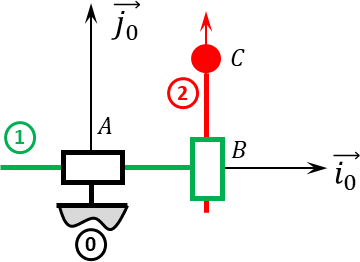
\includegraphics[width=.6\linewidth]{03_TT_01}
\end{center}
\fi

\question{Exprimer les torseurs cinétiques $\torseurci{1}{0}$ et $\torseurci{2}{0}$.}
\ifprof
\else
\fi

\question{Exprimer les torseurs dynamiques $\torseurdyn{1}{0}$ et $\torseurdyn{2}{0}$ en $B$.}
\ifprof
\else
\fi

\question{En déduire $\torseurdyn{1+2}{0}$ en $B$.}
\ifprof
\else
\fi

\ifprof
\else
\begin{flushright}
\footnotesize{Corrigé  voir \ref{C2:08:03}.}
\end{flushright}%
\fi